\section{Assignment Description: The AQNet Network and Its Asynchronous Mechanism}

\subsection{Introduction to the AQNet System}
The system our group chose to model and evaluate is AQNet - Asynchronous Queuing Network Simulator. It is a Multi-Hop Packet-Switched Network, works with a Non-blocking Store-and-Forward mechanism.

In modern communication networks, a node (router or switch) may have to wait until the next node is ready before it can send a packet. This can cause deadlock or network-wide congestion. To solve this problem, AQNet uses a non-blocking communication model. Receiving a packet and processing or forwarding it are fully separated. When a packet arrives, the node immediately records it in the output buffer. Then it hands control back to the system (the event loop or scheduler), so the system can keep receiving other packets. The packet waits in the buffer. It is sent only when the output port (the transmission channel) is idle, and this happens asynchronously.

We chose this problem because it is a natural and practical setting. It allows us to combine and verify all six single-queue models required by the project: $M/M/1$, $M/M/1/K$, $M/M/\infty$, $M/M/n/n$, $M/M/c$, and $M/M/c/K$.


\subsection{Topology and Packet Flow}
AQNet is an open queuing network with no physical feedback loop. It has five functional nodes (N1 to N4 and L1), connected in series and in branches. It also has one independent node, which serves as a reference. A packet travels through the network as follows.
\begin{itemize}
    \item \textbf{Generation at the source (SRC):} Packets are generated independently at \texttt{SRC} by a random process. They then enter the network.
    \item \textbf{Hop 1 - Edge router N1 ($M/M/1/K$ model):} The packet enters the edge access node N1. This node has a single transmission port ($c=1$) and a finite buffer of size $K$. If a packet arrives when the buffer already holds $K$ packets, it is dropped immediately (tail-drop).
    \item \textbf{Hop 2 --- Optical propagation delay L1 ($M/M/\infty$ model):} After N1 sends the packet out, it travels along the physical link L1. On this link, packets travel independently and do not compete for resources. This is equivalent to having infinitely many servers. The packet only experiences a fixed propagation delay before it reaches the next destination.
    \item \textbf{Hop 3 --- Core switch N2 ($M/M/c/K$ model, the bottleneck):} After leaving L1, the packet enters the network core at N2. Here, $c$ parallel service channels share one finite buffer of size $K$. Heavy traffic converges at this node, so it is considered the main bottleneck of the whole network. It determines the throughput and the highest packet loss rate.
    \item \textbf{Hop 4 --- Branching (routing):} After leaving N2, the packet does not follow a single path. The router splits the load by independent probabilities:
    \begin{itemize}
        \item \textbf{Branch A (probability $p = 0.6$)} goes to N3 ($M/M/n/n$ model). N3 acts as a trunking system (or load balancer) with $n$ channels that serve packets directly. It has no waiting buffer. If a packet arrives when all $n$ channels are busy, the packet is rejected immediately (an Erlang loss system).
        \item \textbf{Branch B (probability $p = 0.4$)} goes to N4 ($M/M/c$ model). N4 is a local access switch with $c$ service channels and a very large buffer, which is assumed to be infinite. Buffer overflow does not occur.
    \end{itemize}
     \item \textbf{End at the destination (SNK):} Packets that get through N3 or N4 reach the destination \texttt{SNK}. They complete their life cycle and leave the system.
     \item \textbf{Baseline model ($M/M/1$):} To isolate the system for theoretical analysis, we design a separate $M/M/1$ node with an infinite buffer. It runs in parallel with the network. It serves as a reference for comparing delay and throughput in the ideal case, when there is no congestion.
\end{itemize}


\subsection{Asynchronous Features and Task Lifecycle Management}
To keep the system non-blocking, all processing in AQNet is carried
out through a discrete-event simulation (DES) Scheduler rather than by
waiting on the system (wall-clock) time. Each packet is managed by an
asynchronous task throughout its lifecycle. The table below maps the asynchronous points of the real problem to the modeling mechanisms in AQNet.

\begin{table}[H]
\centering
\begin{tabular}{|p{3.6cm}|p{10cm}|}
\hline
\textbf{Asynchronous Requirement (Real-world Operation)} & \textbf{Processing \& Mapping Mechanism in the AQNet Model} \\
\hline
\textbf{Decoupling Reception from Processing} (Non-blocking I/O) &
The Dispatcher inserts each ``packet arrival'' event into the Priority Queue and immediately returns control, so network nodes are never blocked while waiting for a transmission port. Virtual Time advances only when the Scheduler dequeues the next event for processing, independent of wall-clock time. \\
\hline
\textbf{Message Buffering and Order Preservation} &
Nodes \texttt{N1}, \texttt{N2}, and \texttt{N4} each maintain a dedicated State Queue to hold packets that have not yet been served. The queues follow a strict FCFS (First-Come, First-Served) discipline, ensuring packets are served in order of arrival and thereby preserving causality in the simulation. \\
\hline
\textbf{Possibility of Message Loss} (Packet Loss) &
A packet may be lost in two cases: \newline
1. \textbf{Buffer overflow} at nodes with finite queues (\texttt{N1}, \texttt{N2}): an arriving packet is discarded when the queue is full (Blocking / Tail-drop). \newline
2. \textbf{Immediate rejection} at the bufferless node (\texttt{N3}): if the node is busy upon arrival, the packet is dropped instantly (Erlang Loss). \\
\hline
\textbf{Waiting Time Limit} (Timeout/TTL) &
Each packet is assigned a maximum lifetime (Time-To-Live, TTL). Measured from its entry into the network at \texttt{N1}, if the elapsed time exceeds the TTL before the packet reaches the \texttt{SNK}, the system \textbf{cancels the packet} (Cancelled/Timeout) to release network resources, emulating the Drop Timeout mechanism of IP packets. \\
\hline
\end{tabular}
\caption{Mapping of asynchronous requirements to modeling mechanisms in AQNet}
\label{tab:aqnet-async}
\end{table}




\section{Defining the System Boundary, Services, and Outcomes}
\subsection{System Boundary Diagram}
\begin{figure}[h]
    \centering
    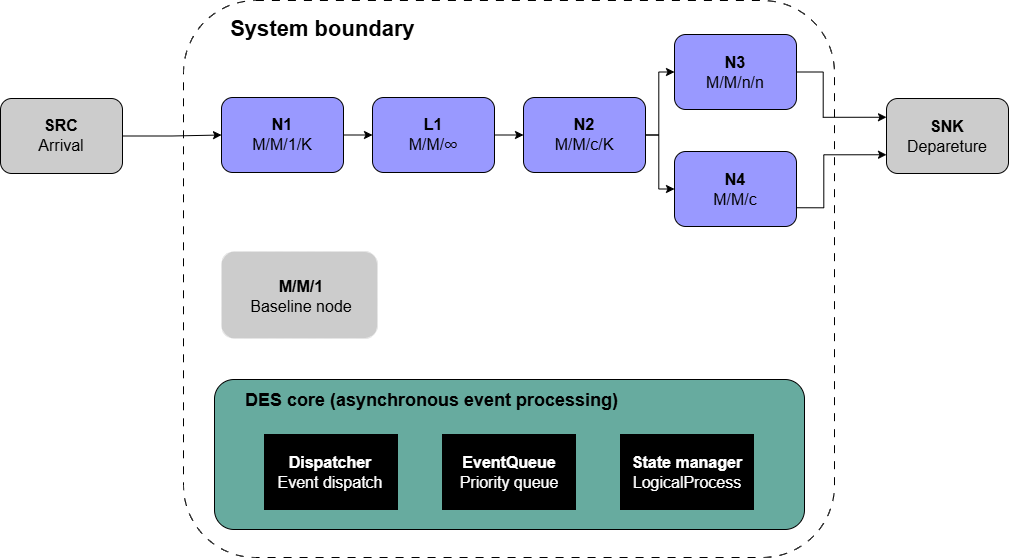
\includegraphics[width=1\textwidth]{graphics/Design1/Sơ đồ Biên hệ thống (System Boundary).drawio.png}
    \caption{System Boundary Diagram}
    \label{fig:ten_hinh}
\end{figure}


\subsection{Service - Outcomes - Corresponding Metrics Table}

\begin{table}[H]
\centering
\footnotesize
\setlength{\tabcolsep}{4pt}
\renewcommand{\arraystretch}{1.15}
{\hyphenpenalty=10000 \exhyphenpenalty=10000 \sloppy
\begin{tabular}{|>{\raggedright\arraybackslash}p{0.22\linewidth}|>{\raggedright\arraybackslash}p{0.06\linewidth}|>{\raggedright\arraybackslash}p{0.15\linewidth}|>{\raggedright\arraybackslash}p{0.25\linewidth}|>{\raggedright\arraybackslash}p{0.18\linewidth}|}
\hline
\textbf{Service} & \textbf{Code} & \textbf{Possible Outcome} & \textbf{Cause} & \textbf{Corresponding Metric} \\
\hline
Asynchronous receiving, buffering, and forwarding of packets through the AQNet network (Store-and-Forward)
& O1 & \textbf{Completed} &
The packet passes successfully through all network nodes (\texttt{N1}, \texttt{L1}, \texttt{N2}, and \texttt{N3}/\texttt{N4}) and safely reaches the Sink. &
M01 ($\rho$), M02 ($L$), M03 ($L_q$), M04 ($W$), M05 ($W_q$), M06 ($X$), M08 (distribution $p_n$), M09 (E2E delay) \\
\cline{2-5}
& O2 & \textbf{Blocked} (buffer full, finite-$K$ systems) &
The packet arrives at a node with a finite queue (\texttt{N1} -- $M/M/1/K$, or \texttt{N2} -- $M/M/c/K$) when the buffer already holds the maximum of $K$ packets, so it is dropped. &
M07 ($P_{block}$) \\
\cline{2-5}
& O3 & \textbf{Rejected} ($M/M/n/n$, all channels busy) &
The packet is routed to the trunking node \texttt{N3}, but all $n$ channels are busy. There is no waiting space, so the service is refused (Erlang loss). &
M07 ($P_{block}$) \\
\cline{2-5}
& O4 & \textbf{TTL expired / Timeout} &
The packet's time in the network exceeds the allowed TTL before it reaches the destination, so the scheduler cancels it. &
M10 (TTL drop rate) \\
\cline{2-5}
& O5 & \textbf{Communication error / Cancelled} &
The event-processing task is deliberately cancelled, or an error occurs in the Future/TaskGroup communication mechanism. &
M11 (counter that records error cases, as defined in Design 2) \\
\hline
\end{tabular}}
\caption{Mapping of services, outcomes, and metrics in AQNet}
\label{tab:aqnet-outcomes}
\end{table}




\section{Mapping Real-World Parameters to Queueing Parameters}
\subsection{Mapping Table of Real-World Parameters to Queueing Parameters}
\noindent To set the input parameters for the simulation, we convert the real network into quantities from queueing theory.

\textbf{Converting real-world figures to get $\mu = 100\text{ pkt/s}$ (standard H6):}
\begin{itemize}
  \item Assume the average packet size in the network is
        $\bar{S} = 1{,}000\text{ bytes} = 8{,}000\text{ bits}$
        (exponentially distributed).
  \item The bandwidth of one standard port or transmission channel is
        $B = 800\text{ kbps} = 800{,}000\text{ bits/s}$.
  \item Then the average service rate of one channel is
        $\mu = \dfrac{B}{\bar{S}} = \dfrac{800{,}000}{8{,}000} = 100\text{ packets/s (pkt/s)}$.
        The average service time of one packet is
        $1/\mu = 10\text{ ms} = 0.01\text{ s}$.
\end{itemize}

\begin{table}[H]
\centering
\small
\begin{tabular}{|p{2.3cm}|p{3.6cm}|p{1.5cm}|p{3.3cm}|p{4.1cm}|}
\hline
\textbf{Queueing Parameter} & \textbf{Real-world Quantity in AQNet} & \textbf{Unit} & \textbf{Value / Range} & \textbf{Modeling Assumption} \\
\hline
$\lambda$ (arrival rate) &
The rate at which packets are generated by the source (\texttt{SRC}) and enter the network. &
pkt/s &
Varies with the load level $\rho \in \{0.3,\ 0.6,\ 0.9\}$. &
The interarrival time follows an exponential distribution (Poisson arrival process). \\
\hline
$\mu$ (service rate) &
The capacity of one network port or one hardware channel to transmit and process packets. &
pkt/s &
Normalized to $\mu = 100\text{ pkt/s}$. &
The packet size (equivalent to the service time) follows an exponential distribution. \\
\hline
$c$ or $n$ (number of servers) &
The number of parallel output ports at the switches \texttt{N2} and \texttt{N4} ($c$), or the number of trunk channels at \texttt{N3} ($n$). &
ports / channels &
$c = 4$ (at \texttt{N2}, \texttt{N4}); $n = 5$ (at \texttt{N3}). &
The parallel ports in the $M/M/c$ model share one common queue (Shared Queue) instead of separate queues. \\
\hline
$K$ (system capacity) &
The buffer capacity at a network port, measured as the maximum number of packets it can hold, including the packet being transmitted. &
packets &
$K \in \{10,\ 20\}$ at the finite nodes. &
A packet that arrives when the buffer is full is dropped immediately (Tail-drop). \texttt{N3} has no buffer ($K = n$). \\
\hline
SD (service discipline) &
The scheduling rule for processing and forwarding packets in the buffer. &
--- &
FCFS (First-Come, First-Served). &
It keeps packets in their order of arrival, as the non-blocking communication system requires. \\
\hline
Topology \& $p_{ij}$ &
The network diagram and the load-splitting (routing) probabilities at the routers. &
--- &
$p_{23} = 0.6$ (via branch A); $p_{24} = 0.4$ (via branch B). &
Routing is probabilistic and independent. It does not depend on the instantaneous congestion of the next nodes. \\
\hline
\end{tabular}
\caption{Mapping of AQNet physical quantities to queueing parameters}
\label{tab:aqnet-params}
\end{table}


\subsection{Discussion of the Markov Assumption in the Model}
\noindent All six required single-queue models in this project are Markovian
($M/M/\dots$). This means arrivals follow a Poisson process and service
times follow an exponential distribution. This assumption gives the system
the \emph{memoryless} property.

\begin{itemize}
  \item \textbf{Justification and benefits:} The Markov assumption is
  necessary in Phases 1 and 2. It allows us to validate the simulation
  results against closed-form analytical formulas, such as Erlang~B,
  Erlang~C, and the product-form solution of Jackson networks. Without the
  memoryless property, we could not use Markov chains to compute the
  reference data.

  \item \textbf{Implications for real-world use:} Real Internet traffic is
  often bursty and self-similar. Packet sizes often follow heavy-tailed
  (Pareto) distributions rather than the exponential distribution. As a
  result, during traffic bursts, the analytical model tends to underestimate
  the real queue length and the packet loss probability
  ($P_{\text{block}}$).

  \item \textbf{Design approach:} Although we use the Markov model as a
  baseline, the AQNet DES architecture remains flexible. The
  \texttt{ArrivalSource} and \texttt{Server} classes accept any specified
  distribution, so we can run experiments with self-similar traffic when
  needed.
\end{itemize}
